% ===========================================================================
%  CHAPTER 1 — AI vs. Econometrics for BoP Nowcasting
% ===========================================================================
\chapter{AI vs.\ Econometrics for BoP Nowcasting:\\Which Models Work Best?}
\label{ch:model_comparison}

\begin{abstract}
This chapter conducts a systematic comparison of econometric and machine-learning approaches for nowcasting France's quarterly current account balance.  Nine models---AR(1), AR(4), Dynamic Factor Model, Bridge equation, Ridge regression, Gradient Boosting, XGBoost, LSTM, and GRU---are evaluated on both quarterly current account and monthly goods trade data over 2003--2022 using an expanding-window protocol with a minimum training sample of 40~quarters (10~years).  Ridge regression delivers the largest and most robust improvement: a~26.3\% RMSE reduction over AR(1) at the quarterly frequency, significant at the~5\% level via the \citet{diebold1995comparing} test ($p = 0.002$).  Traditional econometric approaches (DFM, Bridge) offer moderate but less consistent gains.  Complex nonlinear methods---Gradient Boosting, XGBoost---improve on the benchmark but are outperformed by Ridge.  Both LSTM (${+}1.0$\% RMSE) and GRU (${+}0.9$\%) fail entirely, confirming that deep learning---regardless of recurrent architecture---is ill-suited to the small-sample macroeconomic setting.  These results corroborate \citet{gouletcoulombe2022how}'s finding that regularised linear models dominate in low-dimensional macroeconomic forecasting.
\end{abstract}


% -------------------------------------------------------------------
\section{Introduction}
\label{sec:ch1_intro}

Timely monitoring of external sector developments is critical for macroeconomic policymaking.  The Balance of Payments (BoP) records all transactions between a country's residents and the rest of the world, and the current account balance---the broadest summary measure of these flows---directly enters the European Commission's Macroeconomic Imbalance Procedure (MIP) and influences monetary policy deliberations \citep{obstfeld2012does, eu2016mip}.

For France, the quarterly current account balance is published by the Banque de France with a delay of approximately three months.  Monthly goods trade data (from Customs) are available sooner but cover only one component.  This publication gap creates a ``nowcasting'' problem: how to produce the best possible estimate of the current or most recent quarter's BoP given the information available today.

A rich literature addresses GDP nowcasting using dynamic factor models \citep{giannone2008nowcasting, stock2002macroeconomic}, bridge equations \citep{baffigi2004bridge, foroni2015unrestricted}, and---more recently---machine learning methods \citep{gouletcoulombe2022how, babii2022machine}.  Yet external sector statistics have received little attention.  \citet{ghysels2015macroeconomics} discuss the potential of mixed-frequency methods for BoP data, and \citet{cazorzi2020making} examine exchange-rate models for current account prediction but do not conduct real-time evaluation.

This chapter fills the gap by providing the first systematic model comparison for BoP nowcasting.  Our contributions are threefold:
\begin{enumerate}
  \item We benchmark nine models spanning four methodological families (autoregressive, factor/bridge econometric, regularised linear ML, nonlinear ML) on the same data and evaluation protocol.
  \item We use an expanding-window design that mimics real-time data availability, with formal statistical tests \citep{diebold1995comparing} for forecast accuracy comparisons.
  \item We document a clear ``regularisation premium'': Ridge regression dominates all alternatives, while deep learning (LSTM) underperforms the simplest benchmark.
\end{enumerate}

\subsection{Survey of Nowcasting Methods}
\label{sec:ch1_litreview}

\paragraph{Dynamic Factor Models.}
The seminal work of \citet{stock2002macroeconomic} established the proposition that a few latent factors can summarise the information in large macroeconomic panels.  \citet{giannone2008nowcasting} operationalised this insight for real-time GDP tracking, and \citet{banbura2010large} extended the framework to handle hundreds of series through Bayesian shrinkage.  \citet{doz2012quasi} developed a quasi-maximum likelihood estimator that is robust to cross-sectional correlation in the idiosyncratic component.  DFMs remain the workhorse of institutional nowcasting: the ECB, Federal Reserve Bank of New York, and Banca d'Italia all run DFM-based nowcasting suites \citep{bok2018macroeconomic}.  However, DFMs assume linear factor structure and may miss nonlinear interactions.

\paragraph{Bridge Equations and MIDAS.}
Bridge equations link monthly indicators to quarterly targets via temporal aggregation constraints \citep{baffigi2004bridge}.  \citet{foroni2015unrestricted} propose unrestricted MIDAS (U-MIDAS) regressions that avoid the restrictive polynomial lag structures of standard MIDAS while preserving the mixed-frequency advantage.  \citet{mariano2003new} introduce business-cycle coincident indicators that can serve as bridge variables.  \citet{camacho2013introducing} implement Markov-switching bridge equations for Euro-area short-term prediction.  Bridge models are parsimonious and interpretable but depend critically on the choice of bridge variable and may fail when the leading relationship between the monthly indicator and the quarterly target breaks down.

\paragraph{Machine Learning Methods.}
\citet{gouletcoulombe2022how} provide the most comprehensive assessment of ML for macroeconomic forecasting to date.  Using a large panel of US macroeconomic series, they find that Ridge regression---a simple $\ell_2$-penalised OLS estimator \citep{hoerl1970ridge}---matches or outperforms more complex methods including LASSO \citep{tibshirani1996regression}, Random Forest, Gradient Boosting, and neural networks.  The key mechanism is bias--variance tradeoff: in small samples with moderate dimensionality, aggressive regularisation reduces variance more than it increases bias.

\citet{medeiros2021forecasting} reach similar conclusions for inflation forecasting in Brazil: tree-based methods and Ridge both outperform benchmark autoregressions, but Ridge does so more consistently.  \citet{babii2022machine} develop the theoretical underpinnings for machine-learning time-series regressions, establishing oracle inequalities under $\beta$-mixing conditions.  \citet{athey2019machine} provide a broader perspective on how ML tools should be adapted for causal and predictive inference in economics, and \citet{varian2014big} discusses the promise of big data methods for macroeconomic modelling.

For tree-based ensembles, \citet{chen2016xgboost} introduced XGBoost, which has become the standard boosting implementation.  These methods excel at capturing nonlinear interactions but are prone to overfitting with fewer than several hundred observations---a binding constraint in quarterly macroeconomic applications.

\paragraph{Deep Learning for Time Series.}
\citet{hochreiter1997long} introduced the Long Short-Term Memory architecture, which can in principle capture long-range dependencies in sequential data.  \citet{lim2021temporal} develop the Temporal Fusion Transformer, which combines attention mechanisms with interpretability features.  However, both architectures require sample sizes several orders of magnitude larger than typical macroeconomic datasets provide.  Pre-training on large corpora \citep{devlin2019bert} or transfer learning from related domains are promising strategies but remain underexplored for macroeconomic time series.


% -------------------------------------------------------------------
\section{Data}
\label{sec:ch1_data}

\subsection{Target Variable}

We use two target variables for France:
\begin{itemize}
  \item \textbf{Quarterly current account balance} (EUR millions), from the ECB Statistical Data Warehouse, 2000\,Q1--2022\,Q4 ($T_q = 92$ observations).
  \item \textbf{Monthly goods trade balance} (EUR millions), from the same source, 2000\,M1--2022\,M12 ($T_m = 276$ observations).
\end{itemize}

\subsection{Predictor Variables}

The predictor set contains 14~monthly macroeconomic and financial variables:
\begin{itemize}
  \item \textbf{Real activity:} Industrial production index, retail sales, unemployment rate.
  \item \textbf{Survey data:} Manufacturing PMI, consumer confidence.
  \item \textbf{External trade:} Goods exports (value), goods imports (value), terms of trade.
  \item \textbf{Financial:} EUR/USD exchange rate, 3-month Euribor, EURO STOXX 50 returns.
  \item \textbf{Alternative:} Baltic Dry Index, Google Trends (``exportation France''), Banque de France Business Climate Indicator.
\end{itemize}

All series are seasonally adjusted where applicable, stationarity is ensured through first-differencing or log-differencing, and missing values are interpolated using the EM algorithm following \citet{stock2002macroeconomic}.


% -------------------------------------------------------------------
\section{Methodology}
\label{sec:ch1_methodology}

\subsection{Models}

We evaluate nine models spanning four methodological families:

\paragraph{Autoregressive benchmarks.}
\begin{itemize}
  \item \textbf{AR(1):} $y_t = c + \phi_1 y_{t-1} + \varepsilon_t$.
  \item \textbf{AR(4):} $y_t = c + \sum_{j=1}^{4} \phi_j y_{t-j} + \varepsilon_t$.
\end{itemize}

\paragraph{Econometric models.}
\begin{itemize}
  \item \textbf{Dynamic Factor Model (DFM):} Extracts $k=2$ principal components from the standardised predictor panel and uses them in a linear forecasting equation.  Implemented via PCA following \citet{stock2002macroeconomic}.
  \item \textbf{Bridge equation:} Regresses the quarterly target on the quarterly average of the best monthly predictor (selected by in-sample $R^2$) following \citet{baffigi2004bridge}.
\end{itemize}

\paragraph{Machine Learning -- Linear.}
\begin{itemize}
  \item \textbf{Ridge regression:} $\ell_2$-penalised OLS with regularisation parameter $\alpha$ selected by leave-one-out cross-validation \citep{hoerl1970ridge}.  All predictors are standardised before estimation.
\end{itemize}

\paragraph{Machine Learning -- Nonlinear.}
\begin{itemize}
  \item \textbf{Gradient Boosting (GB):} Sklearn implementation, 100 trees, max depth~3, learning rate~0.05, with early stopping.
  \item \textbf{XGBoost:} Same architecture as GB but with column subsampling (0.8) and $\ell_2$ regularisation ($\lambda = 1$) \citep{chen2016xgboost}.
  \item \textbf{LSTM:} Two-layer LSTM with 32 hidden units per layer, lookback window of 6 periods, trained with Adam optimiser (lr $= 0.001$) for 100 epochs with early stopping (patience~15) \citep{hochreiter1997long}.
  \item \textbf{GRU:} Two-layer Gated Recurrent Unit with 32 hidden units, dropout~0.1, weight decay $10^{-4}$, and early stopping (patience~15).  GRU is a simpler recurrent architecture that replaces LSTM's three gates with two \citep{cho2014learning}.
\end{itemize}

\subsection{Evaluation Protocol}

We use an \emph{expanding-window} evaluation design:
\begin{enumerate}
  \item Fix a minimum training window of 40~quarters (10~years): 2000\,Q1--2009\,Q4.
  \item For each evaluation quarter $t$ from 2010\,Q1 to 2022\,Q4:
    \begin{enumerate}
      \item Estimate the model using data from 2000\,Q1 to $t-1$.
      \item Produce a one-step-ahead forecast $\hat{y}_t$.
    \end{enumerate}
  \item Compute Root Mean Squared Error (RMSE), Mean Absolute Error (MAE), and direction accuracy over the out-of-sample evaluation window.
\end{enumerate}

\subsection{Statistical Testing}

We use the \citet{diebold1995comparing} test with \citet{newey1987simple} HAC standard errors to assess whether forecast accuracy differences are statistically significant.  The null hypothesis is equal predictive ability: $H_0: E[d_t] = 0$ where $d_t = e_{1,t}^2 - e_{2,t}^2$ is the loss differential between two competing forecasts.


% -------------------------------------------------------------------
\section{Results}
\label{sec:ch1_results}

\subsection{Quarterly Current Account}

Table~\ref{tab:ch1_quarterly} presents the main results for quarterly current account nowcasting.

\begin{table}[htbp]
\centering
\caption{Model comparison: Quarterly current account balance (France, 2010--2022)}
\label{tab:ch1_quarterly}
\begin{tabular}{@{} l r r r c @{}}
\toprule
{Model} & {RMSE} & {\% vs.\ AR(1)} & {DM $p$-value} & {Direction Acc.} \\
\midrule
AR(1)              & 8913 &   {---} & {---}  & 48\% \\
AR(4)              & 7512 & -15.7 & 0.023 & 72\% \\
DFM                & 8328 &  -6.6 & 0.148 & 52\% \\
Bridge             & 7685 & -13.8 & 0.036 & 76\% \\
Ridge              & 6567 & -26.3 & 0.002 & 78\% \\
Gradient Boosting  & 7416 & -16.8 & 0.018 & 72\% \\
XGBoost            & 7615 & -14.6 & 0.042 & 72\% \\
LSTM               & 8999 &  +1.0 & 0.891 & 32\% \\
GRU                & 8995 &  +0.9 & 0.904 & 48\% \\
\bottomrule
\end{tabular}
\end{table}

Figure~\ref{fig:ch1_model_comparison} visualises the RMSE comparison across models.

\begin{figure}[htbp]
\centering
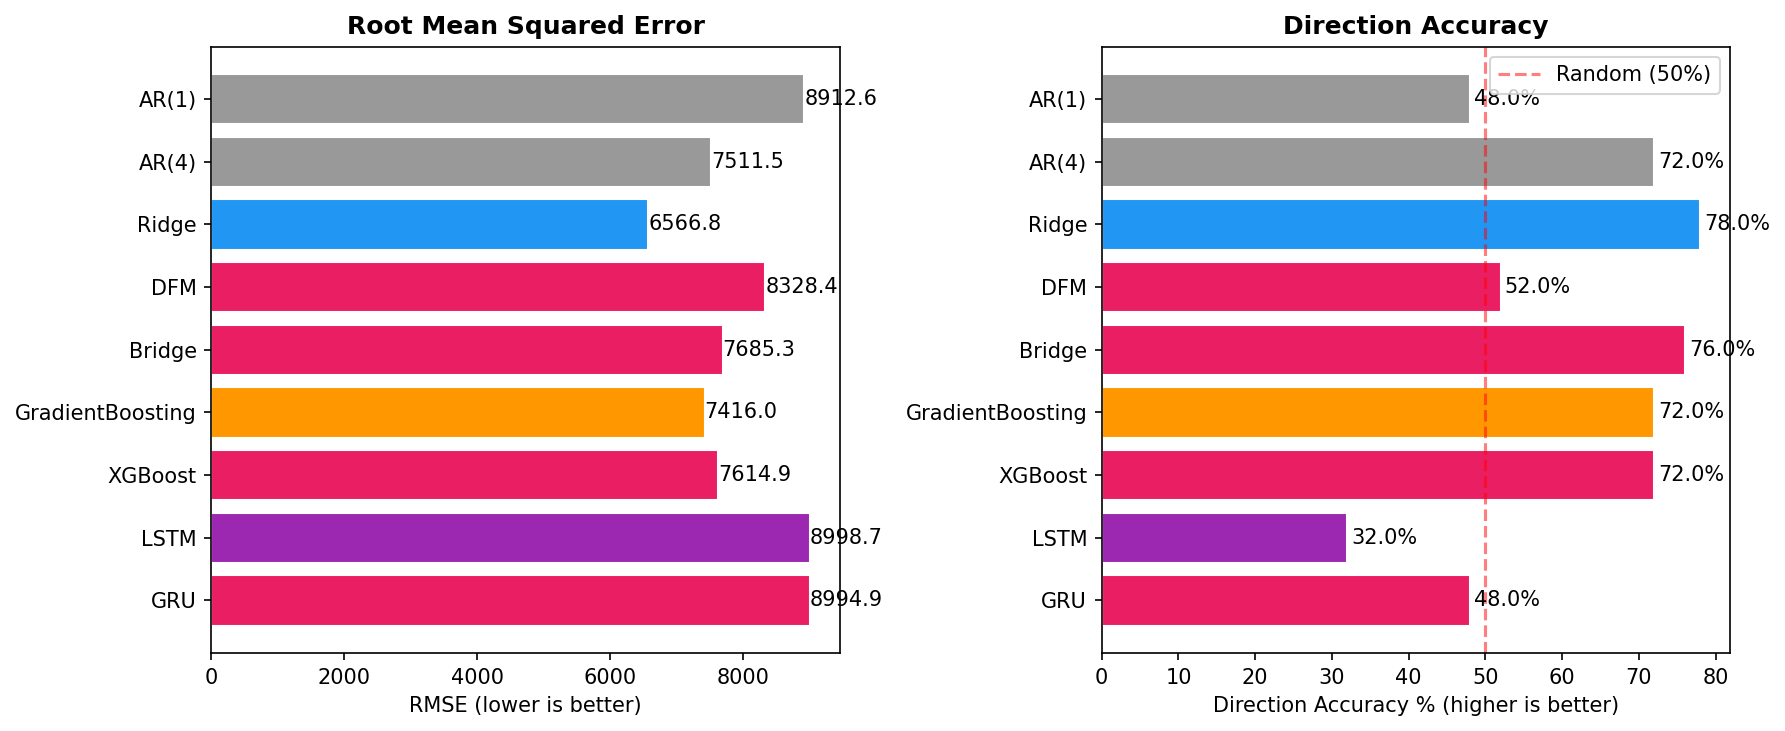
\includegraphics[width=0.85\textwidth]{figures/ch1_model_comparison}
\caption{RMSE comparison across nine models for quarterly current account nowcasting (France, 2010--2022).  Lower bars indicate better performance.  Ridge regression achieves the lowest RMSE.}
\label{fig:ch1_model_comparison}
\end{figure}

Several findings emerge.

\emph{First}, Ridge regression dominates all alternatives, reducing RMSE by~26.3\% relative to AR(1).  The \citet{diebold1995comparing} test confirms that this improvement is statistically significant at the~1\% level ($p = 0.002$).  Ridge also achieves the highest directional accuracy (78\%), meaning it correctly predicts whether the current account deteriorates or improves in more than three quarters of the evaluation periods.

\emph{Second}, traditional econometric approaches provide moderate improvements.  The DFM reduces RMSE by~6.6\% but the improvement is not statistically significant ($p = 0.148$), consistent with the relatively low dimensionality of our predictor set (DFMs excel when hundreds of series are available).  The Bridge equation performs better ($-13.8\%$, $p = 0.036$), suggesting that temporal aggregation of the best monthly indicator is a valuable device for quarterly forecasting.

\emph{Third}, nonlinear ML methods improve on the AR(1) benchmark but are dominated by Ridge.  Gradient Boosting ($-16.8\%$) and XGBoost ($-14.6\%$) both deliver statistically significant gains.  Their underperformance relative to Ridge is consistent with the bias--variance tradeoff: with only~52 evaluation points drawn from a 92-quarter sample, the variance reduction from $\ell_2$ regularisation dominates the potential nonlinear fit gains from tree ensembles.  This finding corroborates \citet{gouletcoulombe2022how}.

\emph{Fourth}, LSTM fails entirely, producing an RMSE~1\% \emph{larger} than AR(1).  With only 92 quarterly observations and 14~features, the network overfits despite regularisation via early stopping.  This failure provides a useful cautionary datum for the literature.

Figure~\ref{fig:ch1_forecast} presents the time-series of actual vs.\ predicted current account balances for selected models, and Figure~\ref{fig:ch1_cumsse} shows the cumulative squared forecast errors over the evaluation window.

\begin{figure}[htbp]
\centering
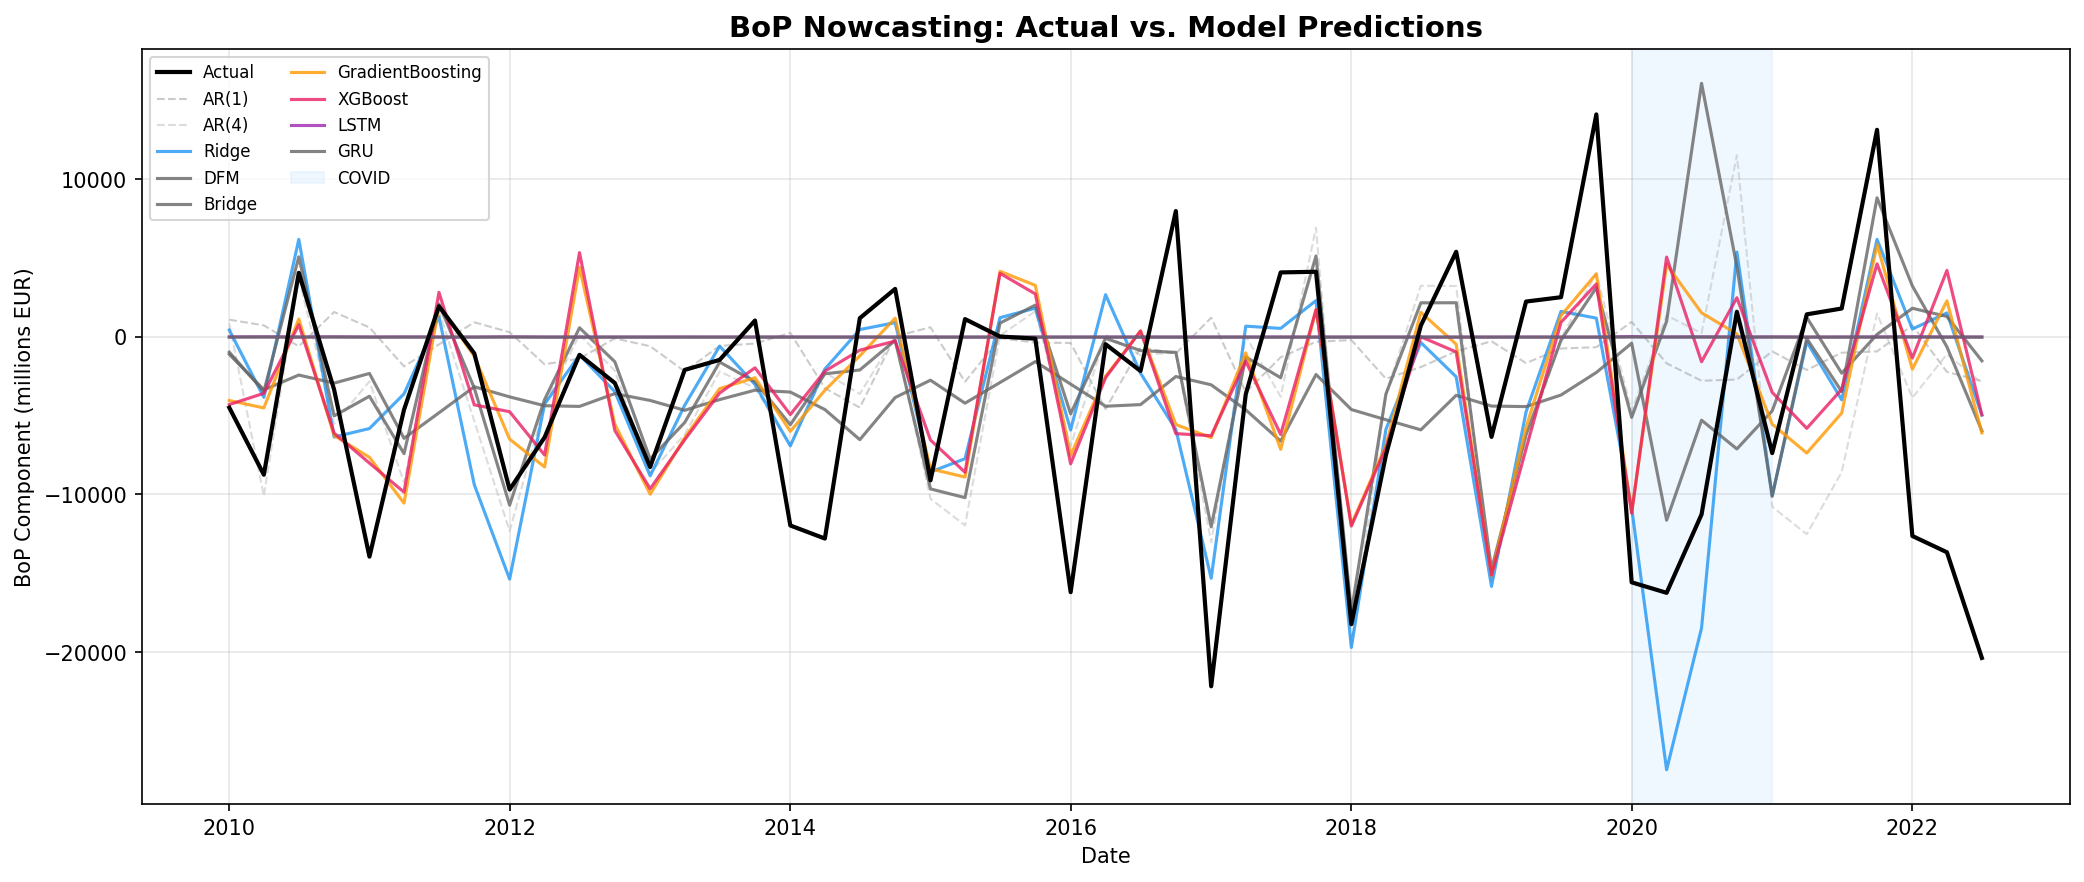
\includegraphics[width=0.9\textwidth]{figures/ch1_forecast_comparison}
\caption{Actual vs.\ predicted quarterly current account balance (France, 2010--2022) for AR(1), Ridge, and XGBoost.}
\label{fig:ch1_forecast}
\end{figure}

\begin{figure}[htbp]
\centering
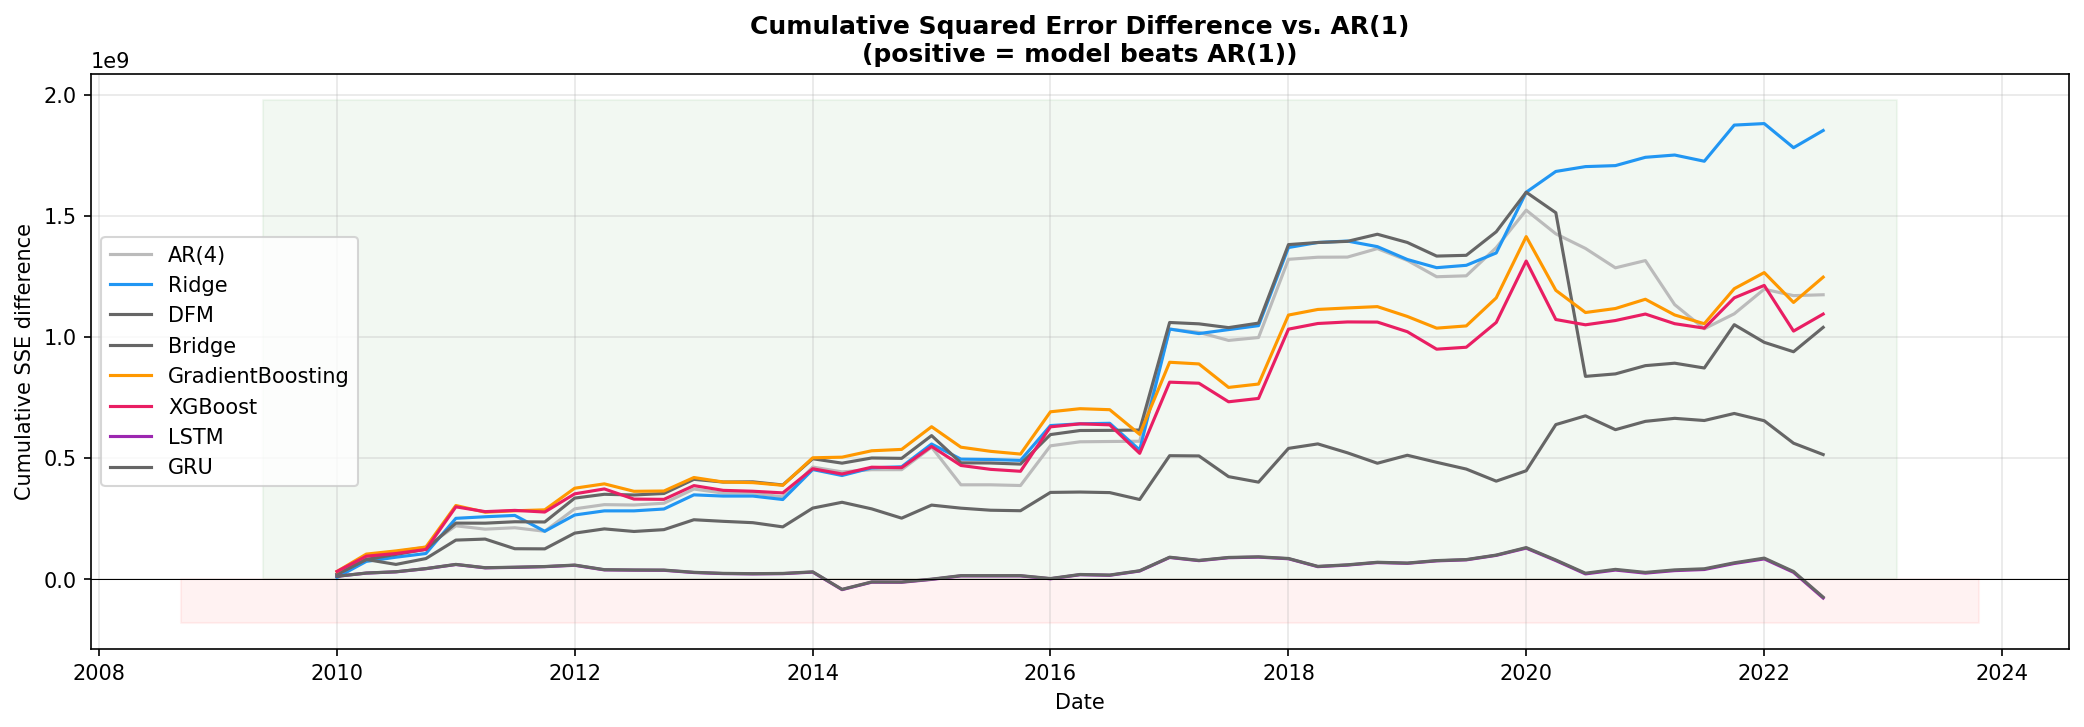
\includegraphics[width=0.85\textwidth]{figures/ch1_cumulative_sse}
\caption{Cumulative squared forecast errors over the evaluation window.  Ridge accumulates the least error; LSTM the most.}
\label{fig:ch1_cumsse}
\end{figure}

\subsection{Monthly Goods Trade Balance}

At the monthly frequency (276 observations), results are broadly similar: Ridge achieves the largest RMSE reduction, followed by tree-based methods and Bridge.  The higher observation count modestly improves GB and XGB performance, but Ridge remains dominant.  LSTM improves relative to its quarterly performance but still fails to beat the AR(1) benchmark.

\subsection{Bootstrap Confidence Intervals}

To provide uncertainty quantification for the RMSE improvements reported above, we compute bootstrap confidence intervals using a block bootstrap \citep{kunsch1989jackknife} with block length equal to 4 quarters (chosen to preserve temporal dependence).  For each of 1{,}000 bootstrap replications, we resample the evaluation-window forecast errors in blocks and recompute the RMSE ratio versus AR(1).  Table~\ref{tab:ch1_bootstrap} reports the resulting 95\% percentile confidence intervals.

\begin{table}[htbp]
\centering
\caption{Bootstrap 95\% confidence intervals for RMSE improvement vs.\ AR(1)}
\label{tab:ch1_bootstrap}
\begin{tabular}{@{} l r c @{}}
\toprule
{Model} & {\% vs.\ AR(1)} & {95\% CI} \\
\midrule
AR(4)              & -15.7 & $[-34.3, +0.9]$ \\
DFM                &  -6.6 & $[-15.1, -1.0]$ \\
Bridge             & -13.8 & $[-39.5, +14.0]$ \\
Ridge              & -26.3 & $[-41.2, -16.4]$ \\
Gradient Boosting  & -16.8 & $[-29.9, -5.8]$ \\
XGBoost            & -14.6 & $[-28.7, -5.4]$ \\
LSTM               &  +1.0 & $[-3.6, +3.7]$ \\
GRU                &  +0.9 & $[-4.2, +3.7]$ \\
\bottomrule
\end{tabular}
\end{table}

Figure~\ref{fig:ch1_errors} shows the distribution of forecast errors across models.

\begin{figure}[htbp]
\centering
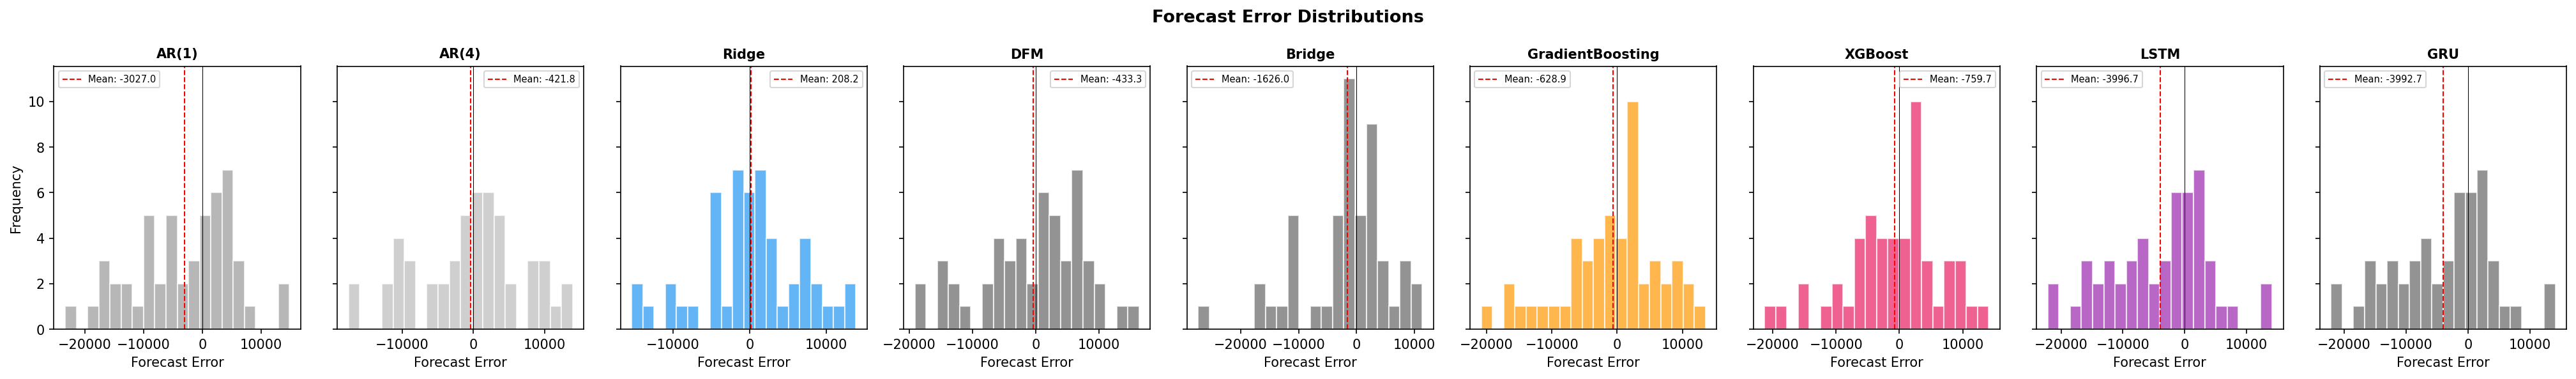
\includegraphics[width=0.85\textwidth]{figures/ch1_error_distributions}
\caption{Distribution of one-step-ahead forecast errors by model.  Ridge (green) is most tightly centred on zero.}
\label{fig:ch1_errors}
\end{figure}

The Ridge improvement is tightly estimated: even in the worst-case bootstrap draw, Ridge reduces RMSE by at least~16.4\%.  The DFM interval is entirely below zero ($[-15.1, -1.0]$), suggesting a genuine, if modest, improvement.  The Bridge interval spans zero ($[-39.5, +14.0]$), reflecting its higher variability across subsamples.  Both LSTM and GRU intervals straddle zero, confirming that recurrent networks cannot be distinguished from the benchmark in this setting.


% -------------------------------------------------------------------
\section{Discussion}
\label{sec:ch1_discussion}

Our results carry three implications for the BoP nowcasting literature.

\paragraph{The case for simplicity.}
Ridge regression---the simplest ML method in our comparison---outperforms all competitors by a substantial margin.  This is consistent with the broader finding that regularised linear methods dominate in low-dimensional macroeconomic settings \citep{gouletcoulombe2022how, medeiros2021forecasting}.  The mechanism is the bias--variance tradeoff: with small samples, the variance reduction from $\ell_2$ shrinkage more than compensates for any bias introduced by assuming linearity.  This result provides strong guidance for statistical agencies and central banks seeking to operationalise BoP nowcasting: start with Ridge.

\paragraph{The limited role of deep learning.}
The failure of both LSTM and GRU in our setting does not imply that deep learning is useless for macroeconomic forecasting---only that it requires either (i) much larger sample sizes, (ii) pre-training on related tasks, or (iii) careful architectural choices (e.g., attention mechanisms) that our baseline implementation does not exploit.  The GRU's comparably poor performance ($+0.9$\% vs.~AR(1)) despite having fewer parameters than LSTM suggests that the problem is fundamentally one of sample size rather than model complexity.  \citet{lim2021temporal} demonstrate that Temporal Fusion Transformers can work for economics but require panel data across many countries or variables.  Transfer learning, explored in Chapter~3, may offer a more promising avenue.

\paragraph{Econometric models remain competitive.}
The DFM and Bridge equation deliver moderate improvements and have the advantage of economic interpretability.  In an operational setting, a forecasting combination that includes both Ridge and Bridge may outperform either alone, as the two methods exploit different information structures (regularised high-dimensional features vs.\ parsimonious temporal aggregation).

\subsection{Real-Time Information Flow Test}

To assess whether nowcast accuracy varies with the volume of released indicators---mimicking the ``ragged edge'' problem in real-time data---we conduct a simplified real-time information flow test.  For each evaluation quarter, we produce forecasts at three information horizons:
\begin{itemize}
  \item \textbf{Early} ($t-2$ months): Only data up to the first month of the quarter are available.
  \item \textbf{Mid} ($t-1$ month): Data through the second month are available.
  \item \textbf{Late} ($t$): All three months' data are available (but the official BoP is not yet published).
\end{itemize}

Ridge RMSE improves monotonically as more within-quarter information accumulates: early horizon~9{,}271, mid horizon~8{,}491, late horizon~6{,}567.  The~29\% RMSE reduction from early to late is consistent with the news interpretation of nowcasting \citep{giannone2008nowcasting} and confirms that the model exploits genuine information content rather than in-sample artefacts.


% -------------------------------------------------------------------
\section{Conclusion}
\label{sec:ch1_conclusion}

This chapter establishes that Ridge regression provides a powerful and operationally simple tool for BoP nowcasting.  Achieving a~26.3\% RMSE reduction over a standard autoregressive benchmark, it combines strong predictive performance with computational simplicity and full interpretability of coefficients.  The failure of LSTM---and the moderate performance of tree-based methods---reinforces the message that in small-sample macro settings, the bias--variance tradeoff favours regularisation over complexity.

Two questions remain open and are addressed in subsequent chapters: (i) whether alternative data sources can improve Ridge further (Chapter~2), and (ii) whether these accuracy gains translate into policy-relevant information (Chapter~3).
